\begin{task}{Lateration\up{+}}{}{}
Follows.
\end{task}
Lateration is a technique for deriving the location of a point in space
by measuring the distance to a number of points, whose location is
known. This technique is used in GNSS systems including GPS, Galieo, or GLONASS
where the distance is measured by signal travel time. Note that in these cases,
in addition to the three unknown coordinates, there is a fourth one representing a
very accurate time. More information on this can be found by searching for Time-of-Arrival
on the Internet.

\begin{center}
  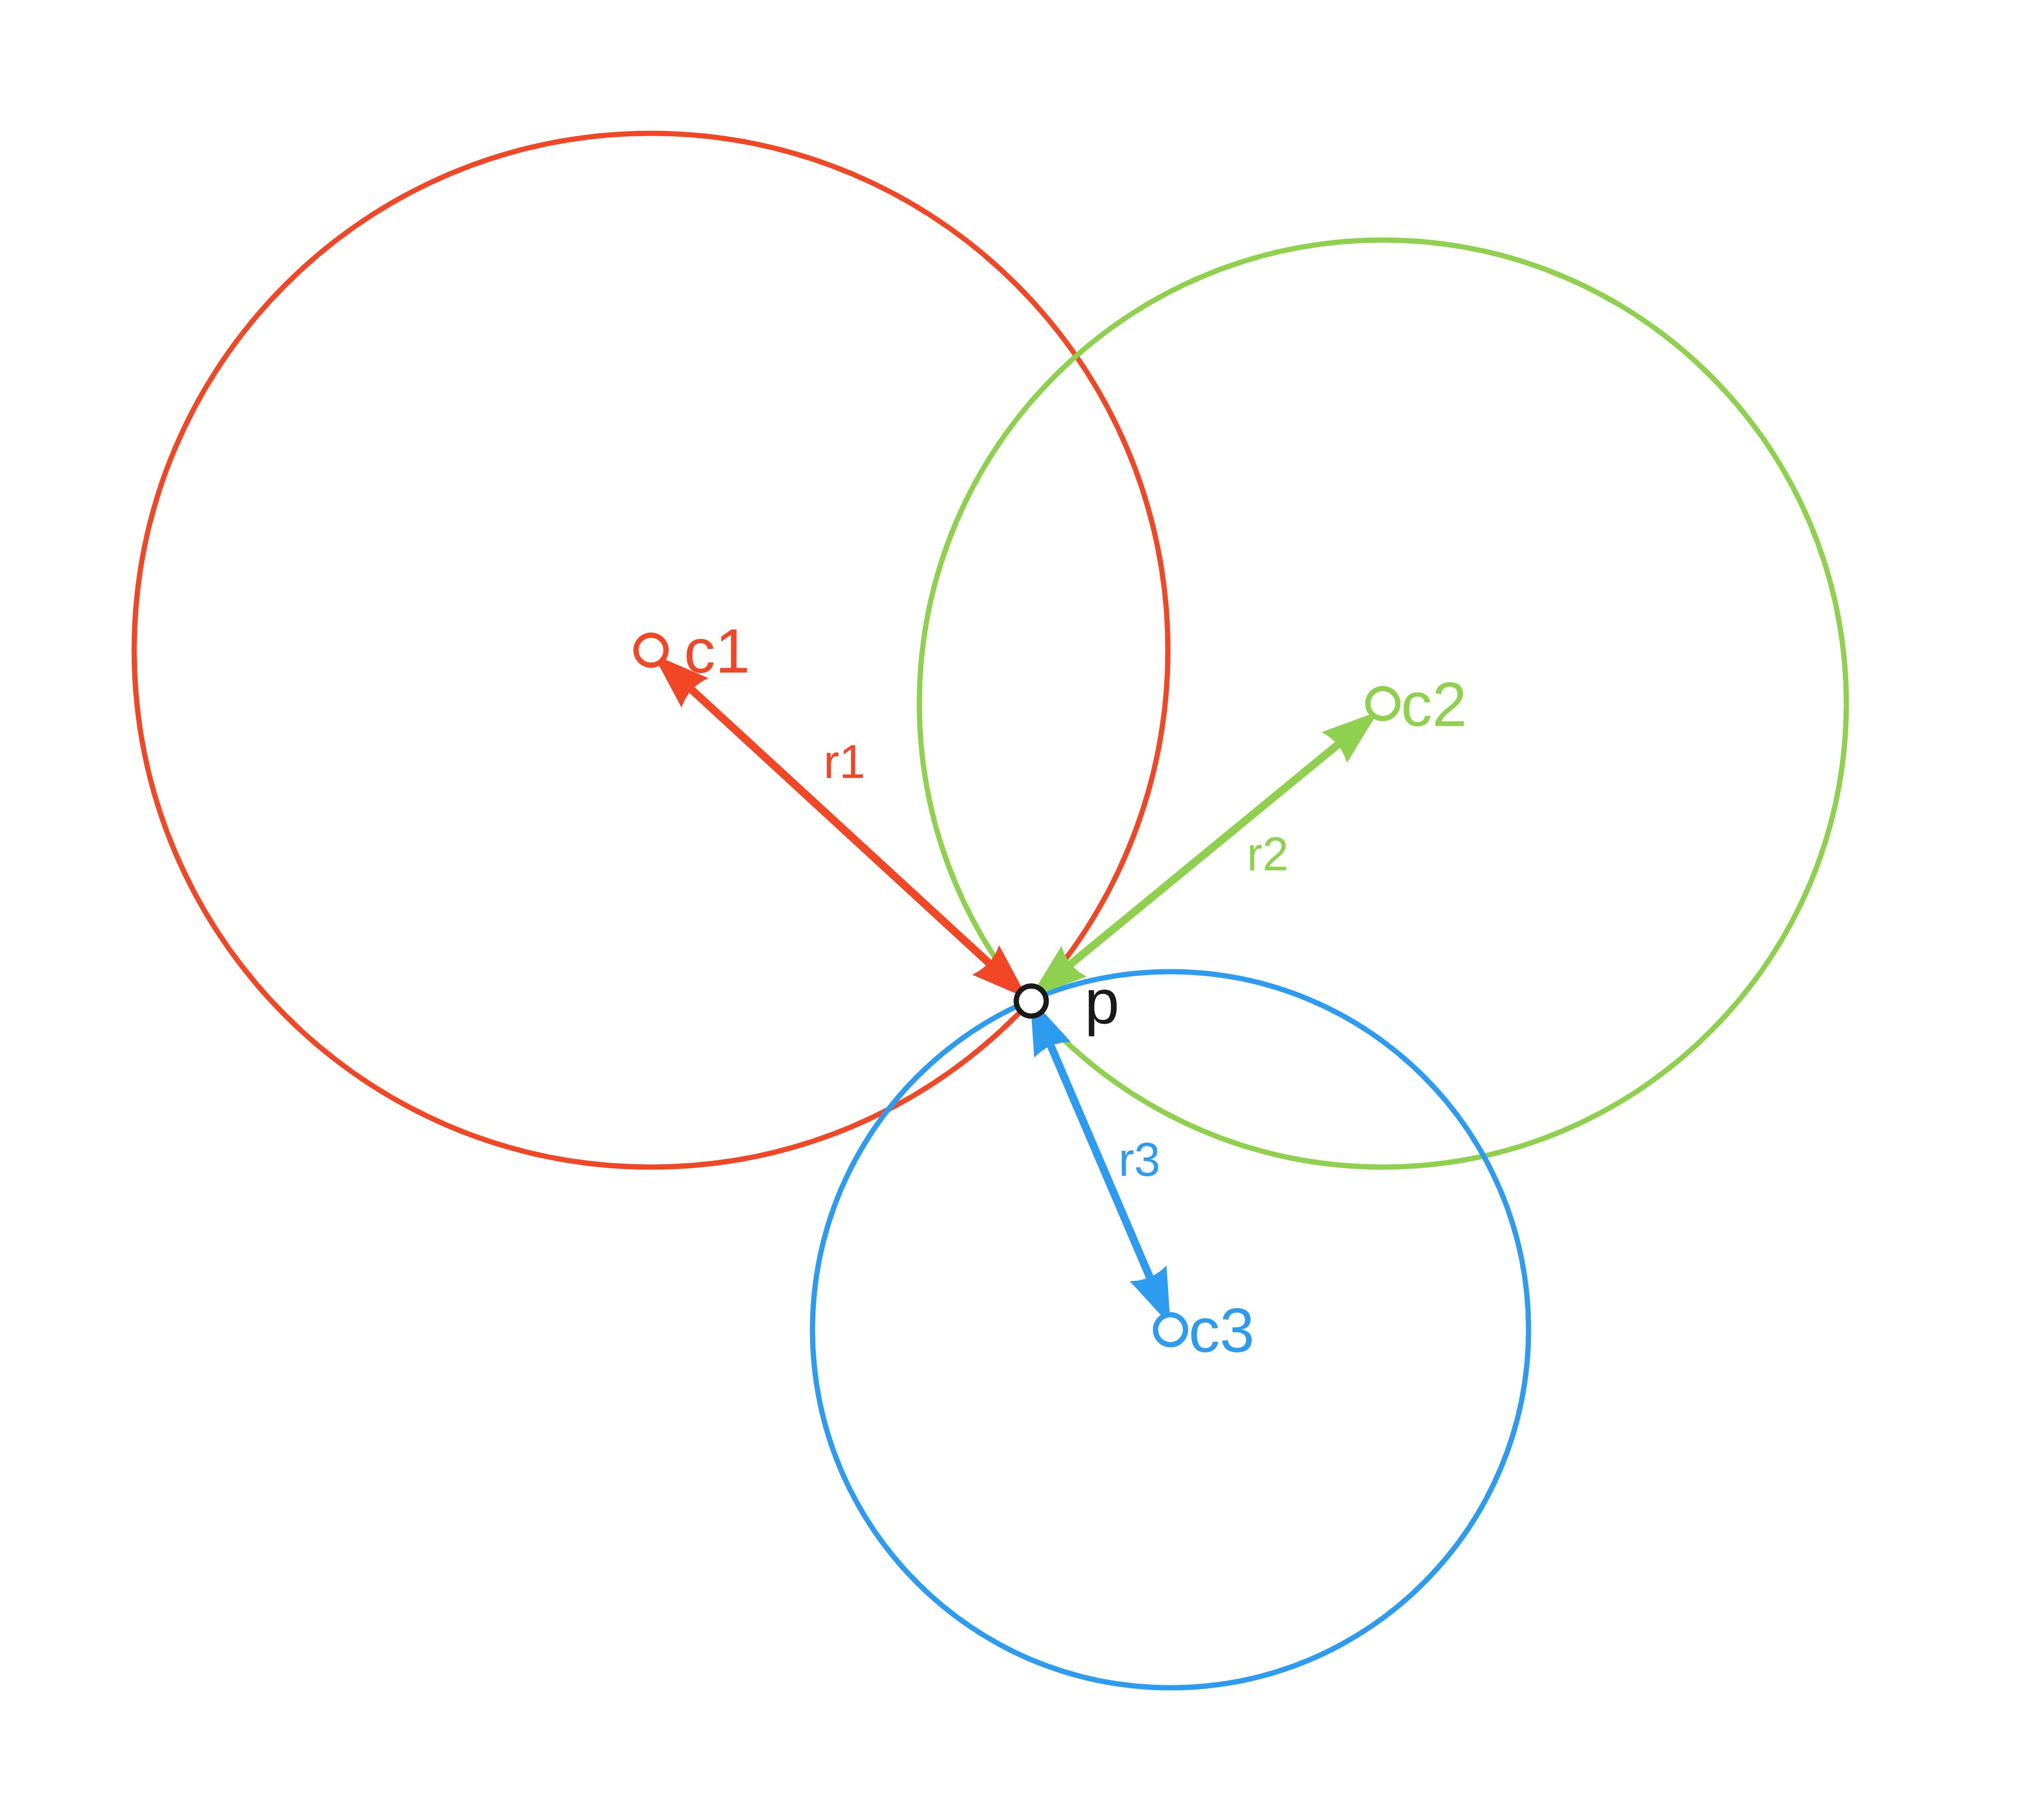
\includegraphics[width=10cm]{gfx/2021_09_laterationsetup.png}
\end{center}
Here \(c_1\), \(c_2\), and \(c_3\) are the the known positions with the
measured radii \(r_1\), \(r_2\), and \(r_3\) And \(p\) is the point we
are looking for.

Put formally the location \(p = (x,y)\) must fulfill all equations
\(k_i\) describing circles around the known centers \(c_i = (x_i, y_i)\)
with measured radii \(r_i\):

\[r_i = k_i(x,y) = \sqrt{(x_i-x)^2 + (y_i-y)^2} i = 1..k\]

This is a
nonlinear problem and therefore the least squares algorithm can not be
used directly. Instead we can use an iterative approach based on
starting with a coarse estimation of the location \(p\). Then we can use
the taylor approximation to linearize the system of equations. This
linearization is only valid around the previous location and can be
solved using the least squares algorithm. The linearization is based on
the following Taylor expansion:

\[
  f(x) = \sum_{i=1..n}{ \frac{f^{i}(x_0)}{i!}(x-x_0)^i + R_{n+1}(x,x_0)}
\]

Here, the Term \(R\) collects the remaining error of using a finite sum.
In order to linearize a system of equations using Taylor expansion, we
can set \(n=1\) and ignore \(R\). For our case of lateration, we need
the partial derivatives in both directions to construct the Taylor sum
as a vector expression. These partial derivatives are given as follows:
\[
  \frac{\partial}{\partial x} k_i(k,y) = - \frac{x_i-x}{\sqrt{(x_i-x)^2+ (y_i -y)^2}}
\]
\[\frac{\partial}{\partial y} k_i(k,y) = - \frac{y_i-y}{\sqrt{(x_i-x)^2+ (y_i -y)^2}}\]

Let now \((\tilde{x}, \tilde{y})\) denote the current estimate of the
location \(p\), then using the measurements \(r_i\) we are left with the
following system of linear equations:

\begin{equation}\label{eq:1}
  r_i = k_i(\tilde{x}, \tilde{y}) + \frac{\partial}{\partial x} k_i(\tilde{x}, \tilde{y})(x - \tilde{x}) + \frac{\partial}{\partial y} k_i(\tilde{x}, \tilde{y})(y - \tilde{y}) i \;= \;1..k
\end{equation}
Introducing the notation \(\hat{x}=x-\tilde{x}\) and
\(\hat{y}=y-\tilde{y}\), we get an overdetermined system of linear
equations for which the least squares method can be applied directly.
This results in a vector expressing a correction of the current location
estimate \((\hat{x}, \hat{y})\) this can be added to the the last
location estimate and the process can be iterated.

\begin{enumerate}
   \item{\textbf{Simple Form of Equation:} Use the values from below and fill in Eqation (\ref{eq:1}). bring it to the
     form \(Ax=b\). What are the values of \(A\) and \(b\)? \newline \emph{When looking closely, you will see that when putting in the constant values for the measurements and the known locations into Equation \ref{eq:1} that only two variables remain. These form together the vector $x = (\hat x, \hat y)$ you want to solve for. The solution is \textbf{not} the location we are after, but due to $\hat x = x - \tilde x$ an offset to improve the current location estimate $\tilde x$ (same for y)}}
   \item{\textbf{Program the Matrix and Constants:} Implement the following procedures:
\begin{lstlisting}[language=MATLAB]
function ret = get_A(tilde_x, tilde_y, C, r)

end

function ret = get_b(tilde_x, tilde_y, C, r)

end
\end{lstlisting}
In this context, the matrix C will hold the known locations, $r$ the measured radii:

\[C= \begin{pmatrix}x_1\;y_1\\x_2\;y_2\\x_3\;y_3\\x_4\;y_4\end{pmatrix}=\begin{pmatrix}0\;0\\10\; 0\\15\;0\\0\;12\end{pmatrix} \;\;  \;\;r = \begin{pmatrix}r_1\\r_2\\r_3\\r_4\end{pmatrix}=\begin{pmatrix}2.92\\8.14\\15.46\\9.89\end{pmatrix}\]
Feel free to simplify the signature by removing parameters you don't need.
   }
   \item{\textbf{Location Estimation:}
Given the previously mentioned set of locations and measurements calculate the
estimated location correction in each step, starting with the initial
location estimate \((\tilde{x},\tilde{y}) =(20,20)\). Report this vector for at least 3 steps.
Then run the program for seven steps and report the final result. Try to implement a version with a \code{while} loop
that stops as soon as the error (as measured by the residuum) does not decrease enough.
   }
\end{enumerate}






